\documentclass[11pt,aspectratio=169]{beamer}
\usepackage{amsmath,amssymb,bm,graphicx}
\usetheme{default}
\setbeamertemplate{navigation symbols}{}
\setbeamertemplate{headline}{}
\setbeamertemplate{footline}{%
  \leavevmode\hbox{%
    \begin{beamercolorbox}[wd=\paperwidth,ht=2.6ex,dp=1.1ex,right]{page number in head/foot}%
      \insertframenumber/\inserttotalframenumber\hspace{0.35cm}
    \end{beamercolorbox}}}
\setbeamertemplate{frametitle}{\vspace{0.25cm}\insertframetitle\par\vspace{0.08cm}\hrule}
\setbeamercolor{normal text}{fg=black,bg=white}
\setbeamercolor{frametitle}{fg=black,bg=white}
\setbeamercolor{structure}{fg=black}
\setbeamersize{text margin left=0.7cm,text margin right=0.7cm}
\graphicspath{{figures/}}
\newcommand{\bx}{\bm x}
\newcommand{\dd}{\mathrm d}
\newcommand{\Vhzero}{\mathcal V_{h,0}}
\newcommand{\uex}{u_{\mathrm{exact}}}

\begin{document}

\begin{frame}
\centering\vfill
{\LARGE\bfseries Nonlinear Finite Element Methods\par}
\vspace{0.45cm}
{\Large Lecture 4: Nonlinear Diffusion and Reaction\par}
\vspace{0.45cm}
Prashant K. Jha\par
ME/BME 736\par
November 12, 2026
\vfill
\end{frame}

\begin{frame}{Lecture outline}
\begin{enumerate}
\item Derive the variational problem and choose the trial and test spaces.
\item Compute the first variation of the potential and linearize the residual.
\item Write the finite element Newton correction equation.
\item Supply the residual and tangent to DOLFINx and compare the solution with a known exact solution.
\end{enumerate}
In the elasticity example, UFL computed the derivatives. Here we take the
first variation of the potential and differentiate the residual with respect
to $u$ by hand.
\end{frame}

\begin{frame}{Strong form on the unit square}
Let $\Omega=(0,1)^2$ and $\bx=(x,y)^T$. Find a scalar field $u$ satisfying
\[
\boxed{
\begin{aligned}
-\nabla\cdot\bigl(k(u)\nabla u\bigr)+c(\bx)u^3
  &=f(\bx) && \text{in }\Omega,\\
u &=0 && \text{on }\partial\Omega,
\end{aligned}}
\qquad
k(u)=k_0(1+\nabla u\cdot\nabla u).
\]
Here $k_0>0$ is constant, and $k(u)$ depends on $\nabla u$.
The reaction coefficient $c$ and the source $f$ are prescribed.
For the weak problem assume
\[
c\in L^\infty(\Omega),\qquad c\ge 0\ \text{a.e. in }\Omega,\qquad
f\in L^{4/3}(\Omega).
\]
\end{frame}

\begin{frame}{Integration by parts}
First suppose $u$ and the test function $v$ are smooth, with
$v=0$ on $\partial\Omega$. Multiply the differential equation by $v$
and integrate:
\[
-\int_\Omega v\,\nabla\cdot(k(u)\nabla u)\,\dd\bx
+\int_\Omega c\,u^3v\,\dd\bx
=\int_\Omega fv\,\dd\bx .
\]
Integrate the diffusion term by parts, using the outward unit normal $\bm n$:
\[
\int_\Omega k(u)\nabla u\cdot\nabla v\,\dd\bx
-\int_{\partial\Omega} v\,k(u)\nabla u\cdot\bm n\,\dd s
+\int_\Omega c\,u^3v\,\dd\bx
=\int_\Omega fv\,\dd\bx .
\]
The boundary integral is zero because $v=0$ there.
The remaining terms need only first derivatives of $u$ and $v$.
\end{frame}

\begin{frame}{H\"older's inequality}
To choose the trial and test spaces, we need to know when the products
in the integrals are integrable.

\medskip
Let $1\le p,q\le\infty$ with $1/p+1/q=1$, taking $1/\infty=0$.
If $g\in L^p(\Omega)$ and $h\in L^q(\Omega)$, then $gh\in L^1(\Omega)$ and
\[
\boxed{\int_\Omega |gh|\,\dd\bx
  \le \|g\|_{L^p(\Omega)}\|h\|_{L^q(\Omega)}.}
\]
For three factors, let $1\le p,q,r\le\infty$ with $1/p+1/q+1/r=1$.
If $g\in L^p(\Omega)$, $h\in L^q(\Omega)$, and $j\in L^r(\Omega)$,
then $ghj\in L^1(\Omega)$ and
\[
\boxed{\int_\Omega |ghj|\,\dd\bx
  \le \|g\|_{L^p(\Omega)}\|h\|_{L^q(\Omega)}\|j\|_{L^r(\Omega)}.}
\]
\end{frame}

\begin{frame}{Trial and test spaces}
Use the same space for $u$ and $v$ because the prescribed boundary value is zero:
\[
V=W^{1,4}_0(\Omega)
=\{z\in W^{1,4}(\Omega):z=0\ \text{on }\partial\Omega\}.
\]
The trace of $z$ on $\partial\Omega$ is zero, and $z,\nabla z\in L^4$.

The nonlinear diffusion flux $k_0|\nabla u|^2\nabla u$ is in $L^{4/3}$
because $(|\nabla u|^3)^{4/3}=|\nabla u|^4$.
H\"older's inequality with $p=4/3$ and $q=4$ gives
\[
\begin{aligned}
\int_\Omega |\nabla u|^3|\nabla v|\,\dd\bx
  &\le \|\nabla u\|_{L^4}^3\|\nabla v\|_{L^4},\\
\int_\Omega |cu^3v|\,\dd\bx
  &\le \|c\|_{L^\infty}\|u\|_{L^4}^3\|v\|_{L^4},\\
\int_\Omega |fv|\,\dd\bx
  &\le \|f\|_{L^{4/3}}\|v\|_{L^4}.
\end{aligned}
\]
All norms are finite: $u,v\in V$, $c\in L^\infty$, and $f\in L^{4/3}$.
The Banach space $V$ requires $L^4$ gradients. The Hilbert space $H^1_0$ does not.
\end{frame}

\begin{frame}{Variational problem and residual}
For $u,v\in V$ define
\[
\begin{aligned}
a(u;v)&=\int_\Omega
 \bigl[k(u)\nabla u\cdot\nabla v+c\,u^3v\bigr]\,\dd\bx,\\
\ell(v)&=\int_\Omega fv\,\dd\bx.
\end{aligned}
\]
The form $a(u;v)$ is nonlinear in $u$ and linear in $v$.
The variational problem is to find $u\in V$ such that
\[
\boxed{a(u;v)=\ell(v)\qquad\text{for every }v\in V.}
\]
Use the same residual convention as in nonlinear elasticity:
\[
R(u;v)=\ell(v)-a(u;v).
\]
\end{frame}

\begin{frame}{Total potential and the first variation}
For $u\in V$ define
\[
\Pi(u)=\int_\Omega\left[
\frac{k_0}{2}|\nabla u|^2+\frac{k_0}{4}|\nabla u|^4
+\frac{c}{4}u^4-fu
\right]\,\dd\bx,\qquad |\nabla u|^2=\nabla u\cdot\nabla u.
\]
The gradient terms are integrable because $\nabla u\in L^4$ and
$L^4(\Omega)\subset L^2(\Omega)$ on the square.
The reaction energy is integrable since $u\in L^4$ and $c$ is bounded.
For the load, $\int_\Omega |fu|\,\dd\bx\le \|f\|_{L^{4/3}}\|u\|_{L^4}$.
Both norms are finite since $f\in L^{4/3}$ and $u\in V\subset L^4$.

\medskip
For any $v\in V$, the perturbed field $u+\varepsilon v$ still satisfies
the boundary condition. The first variation is
\[
\delta\Pi(u;v)=
\left.\frac{\dd}{\dd\varepsilon}\Pi(u+\varepsilon v)\right|_{\varepsilon=0}.
\]
\end{frame}

\begin{frame}{First variation gives the negative residual}
In $\Pi(u+\varepsilon v)$, the squared gradient is
\[
|\nabla(u+\varepsilon v)|^2
=|\nabla u|^2+2\varepsilon\,\nabla u\cdot\nabla v
+\varepsilon^2|\nabla v|^2 .
\]
For the quartic gradient term, the chain rule gives
\[
\left.\frac{\dd}{\dd\varepsilon}
\frac{k_0}{4}|\nabla(u+\varepsilon v)|^4\right|_{\varepsilon=0}
=\frac{k_0}{4}\,2|\nabla u|^2(2\nabla u\cdot\nabla v).
\]
Differentiating all four terms gives
\[
\begin{aligned}
\delta\Pi(u;v)
&=\int_\Omega\bigl[k_0\nabla u\cdot\nabla v
+k_0|\nabla u|^2\nabla u\cdot\nabla v+cu^3v-fv\bigr]\,\dd\bx\\
&=a(u;v)-\ell(v)=-R(u;v).
\end{aligned}
\]
Thus stationarity in every direction $v\in V$ gives
$a(u;v)=\ell(v)$ for every $v\in V$.
\end{frame}

\begin{frame}{Variation of the diffusion and reaction terms}
Hold $v\in V$ fixed and perturb $u\in V$ in the direction $w\in V$:
\[
\delta_u R(u;v)[w]=
\left.\frac{\dd}{\dd\varepsilon}R(u+\varepsilon w;v)\right|_{\varepsilon=0}.
\]
The load term does not vary with $u$. In the diffusion term,
\[
\begin{aligned}
\left.\frac{\dd}{\dd\varepsilon}k(u+\varepsilon w)\right|_{\varepsilon=0}
  &=2k_0\nabla u\cdot\nabla w,\\
\left.\frac{\dd}{\dd\varepsilon}\bigl[k(u+\varepsilon w)\nabla(u+\varepsilon w)\bigr]\right|_{\varepsilon=0}
  &=k(u)\nabla w+2k_0(\nabla u\cdot\nabla w)\nabla u .
\end{aligned}
\]
In the reaction term the corresponding derivative is
$\left.\frac{\dd}{\dd\varepsilon}\bigl[c(u+\varepsilon w)^3\bigr]\right|_{\varepsilon=0}=3cu^2w$.

Since $\delta\Pi=-R$, the tangent $\delta_uR$ is the negative of the second variation of $\Pi$.
\end{frame}

\begin{frame}{Derivative of the residual}
Differentiate $R=\ell-a$ using the diffusion and reaction derivatives:
\[
\boxed{\begin{aligned}
\delta_u R(u;v)[w]=-\int_\Omega\bigl[&
 k(u)\nabla w\cdot\nabla v\\
 &+2k_0(\nabla u\cdot\nabla w)(\nabla u\cdot\nabla v)
 +3cu^2wv\bigr]\,\dd\bx.
\end{aligned}}
\]
Use H\"older's inequality with exponents $2,4,4$, since $1/2+1/4+1/4=1$:
\[
\begin{aligned}
\int_\Omega|\nabla u|^2|\nabla w||\nabla v|\,\dd\bx
&\le \|\nabla u\|_{L^4}^2\|\nabla w\|_{L^4}\|\nabla v\|_{L^4},\\
\int_\Omega |cu^2wv|\,\dd\bx
&\le \|c\|_{L^\infty}\|u\|_{L^4}^2\|w\|_{L^4}\|v\|_{L^4}.
\end{aligned}
\]
The squares $|\nabla u|^2$ and $u^2$ are in $L^2$ because $u\in V$.
Since $w,v\in V$, the $L^4$ norms of $w,v,\nabla w,\nabla v$ are finite.
The norm $\|c\|_{L^\infty}$ is finite by assumption.

\end{frame}

\begin{frame}{Newton correction and update}
At the current iterate $u^k$, use the first-order approximation
\[
R(u^k+\Delta u^k;v)\approx
 R(u^k;v)+\delta_u R(u^k;v)[\Delta u^k].
\]
We want the residual at $u^k+\Delta u^k$ to vanish for every $v\in V$.
In Newton's method, we set its first-order approximation to zero.
Now restrict this equation to
$\Vhzero\subset V$, the continuous piecewise-linear space on a triangular
mesh with zero boundary values. Starting with $u_h^0=0$, at step $k$ find
$\Delta u_h^k\in\Vhzero$ such that
\[
\delta_u R(u_h^k;v_h)[\Delta u_h^k]=-R(u_h^k;v_h)
\qquad \text{for every }v_h\in\Vhzero.
\]
For a full Newton step, set $u_h^{k+1}=u_h^k+\Delta u_h^k$.
Both $u_h^k$ and $\Delta u_h^k$ vanish on $\partial\Omega$, so the update
preserves the boundary condition.
\end{frame}

\begin{frame}{The linear problem at each iteration}
For the correction, substitute $u=u_h^k$, $w=\Delta u_h^k$ and $v=v_h$
in the tangent and multiply both sides of the Newton equation by $-1$:
\[
\begin{aligned}
\int_\Omega\bigl[&
 k(u_h^k)\nabla\Delta u_h^k\cdot\nabla v_h\\
 &+2k_0(\nabla u_h^k\cdot\nabla\Delta u_h^k)(\nabla u_h^k\cdot\nabla v_h)
 +3c(u_h^k)^2\Delta u_h^k v_h\bigr]\,\dd\bx
 =R(u_h^k;v_h).
\end{aligned}
\]
With $u_h^k$ fixed, the left side is bilinear in the correction and test
function. Taking $v_h=\Delta u_h^k$ gives a lower bound of
$k_0\|\nabla\Delta u_h^k\|_{L^2}^2$. The other terms are nonnegative because
$k_0>0$ and $c\ge 0$.
A nonzero correction with zero boundary values cannot have zero gradient.
The matrix on the free degrees of freedom is symmetric positive definite,
so the correction is unique.
\end{frame}

\begin{frame}{FEniCSx example: mesh and data}
\begin{columns}[onlytextwidth,T]
\begin{column}{0.55\textwidth}
Use $k_0=1$ and $c(x,y)=1+x$ on the unit square.
Choose a known solution that vanishes on all four edges:
\[
\uex(x,y)=4x(1-x)y(1-y).
\]
Substitute $\uex$ for $u$ on the left of the PDE and use the result as $f$:
\[
\begin{aligned}
f={}&-\nabla\cdot\bigl[k(\uex)\nabla\uex\bigr]\\
&+c\,\uex^3.
\end{aligned}
\]
Use 288 triangles and impose $u_h=0$ on every exterior edge.
\end{column}
\begin{column}{0.42\textwidth}
\centering
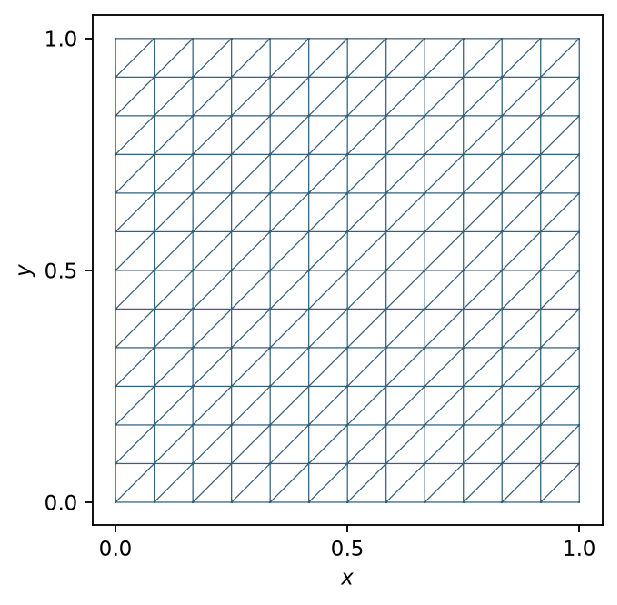
\includegraphics[width=0.94\textwidth]{nonlinear_diffusion_mesh.pdf}
\end{column}
\end{columns}
\end{frame}

\begin{frame}[fragile]{Residual and tangent in UFL}
In the notebook, \texttt{g}, \texttt{gv}, and \texttt{gw} are the gradients
of \texttt{u}, \texttt{v}, and \texttt{w}. Here \texttt{k} is the diffusion
coefficient evaluated at the current iterate.
\begin{verbatim}
residual = (f * v - k * ufl.dot(g, gv) - c * u**3 * v) * dx
tangent = -(
    k * ufl.dot(gw, gv)
    + 2 * k0 * ufl.dot(g, gw) * ufl.dot(g, gv)
    + 3 * c * u**2 * w * v
) * dx
\end{verbatim}
The minus sign in \texttt{tangent} comes from differentiating $R=\ell-a$.
\end{frame}

\begin{frame}[fragile]{Nonlinear solve in DOLFINx}
Pass $R$, $\delta_uR$, and the zero boundary condition to \texttt{NonlinearProblem}.
DOLFINx assembles the forms, and PETSc solves the nonlinear system.
\begin{verbatim}
problem = NonlinearProblem(
    residual, u, bcs=[bc], J=tangent,
    petsc_options_prefix="diffusion_", petsc_options=solver_options,
)
problem.solve()
\end{verbatim}
The notebook starts from zero and uses Newton with backtracking and a
direct solve for each correction equation. Backtracking may shorten the
update without changing the correction equation.

\medskip
Companion notebook: \path{notebooks/nonlinear/nonlinear_diffusion_reaction.ipynb}
\end{frame}

\begin{frame}{Computed and exact solutions}
\centering
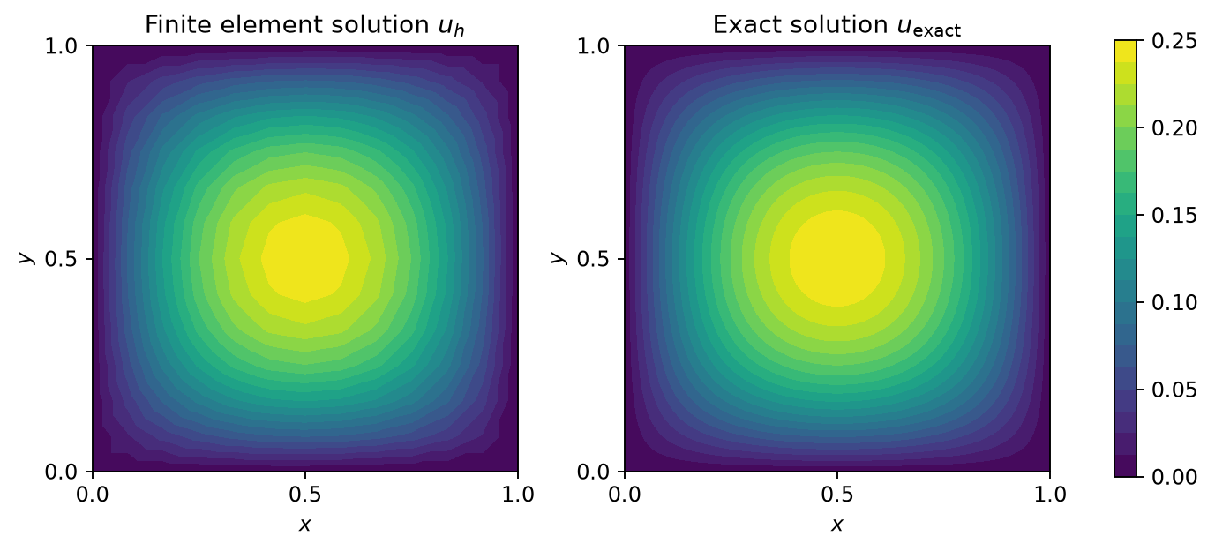
\includegraphics[width=0.88\textwidth]{nonlinear_diffusion_solution.pdf}\par
\medskip
Newton iterations: 7. \quad
$\|u_h-\uex\|_{L^2(\Omega)}=2.1808\times10^{-3}$.
\end{frame}

\begin{frame}{Summary}
\begin{itemize}
\item Both trial and test functions are in $W^{1,4}_0(\Omega)$. Continuous
$P_1$ functions with zero boundary values belong to this space because their
gradients are piecewise constant.
\item The first variation is $\delta\Pi(u;v)=-R(u;v)$. To obtain the
tangent, vary $u$ while holding $v$ fixed.
\item At a fixed iterate, the Newton equation is linear in the correction.
Supply $R$ and its derivative $\delta_uR$ to the nonlinear solver.
\end{itemize}
\end{frame}

\end{document}
